\documentclass{beamer}
\usetheme{default}
\usecolortheme{seahorse}
\usepackage[utf8]{inputenc}
\usepackage{graphicx}
\usepackage{booktabs}
\usepackage{amsmath}
\usepackage{natbib}
\usepackage[italian]{babel}
\usepackage{hyphenat}
\hyphenation{mate-mati-ca recu-perare}
\usepackage{tikz}
\usetikzlibrary{shapes,arrows.meta,positioning}

\title[Lezione 1]{Hello, Psychometrics!}
\subtitle{Master Avanzato in Economia e Politica Agraria}
\author{Giovanbattista Califano}
\date[Portici, 20 e 23/04/2026]{Scale Attitudinali per lo Studio \\ delle Preferenze del Consumatore \\ 20 e 23 Aprile 2026}
\institute[UNINA]{Università degli Studi di Napoli Federico II, giovanbattista.califano@unina.it}

\AtBeginSection[]
{
  \begin{frame}<beamer>
    \frametitle{Passiamo a...}
    \tableofcontents[currentsection]
  \end{frame}
}

\begin{document}

\frame{\titlepage}

\begin{frame}{Tabella di marcia}
    \begin{center}
        \begin{tabular}{|l|l|c|}
        \hline
        20/04 e 23/04 &  Hello, Psychometrics! & $\bigcirc$ \\
        \hline
        24/04 & Affidabilità e Validità di una Misura & $\bigcirc$ \\
        \hline
        24/04 e 27/04 & Variabili Latenti: Riflessive o Formative? & $\bigcirc$ \\
        \hline
        30/04 e 07/05 & Modelli ad Equazioni Strutturali & $\bigcirc$ \\
        \hline
        \end{tabular}
    \end{center}
\vspace{0.1cm}
\footnotesize
Riferimenti consigliati: \\
\begin{itemize}
    \item Capitoli 4 e 7 da \cite{jhangiani2019research}
    \item Capitoli 7, 10 e 14 da \cite{olivero2022psicologia}
    \item Capitolo 12 da \cite{mehmetoglu2022applied}
\end{itemize}
\scriptsize
\bibliographystyle{apalike}
\bibliography{text}
\end{frame}

\begin{frame}{Perché la psicometria? Il caso del dott. Mirko Marmellata}
\begin{figure}
    \centering
    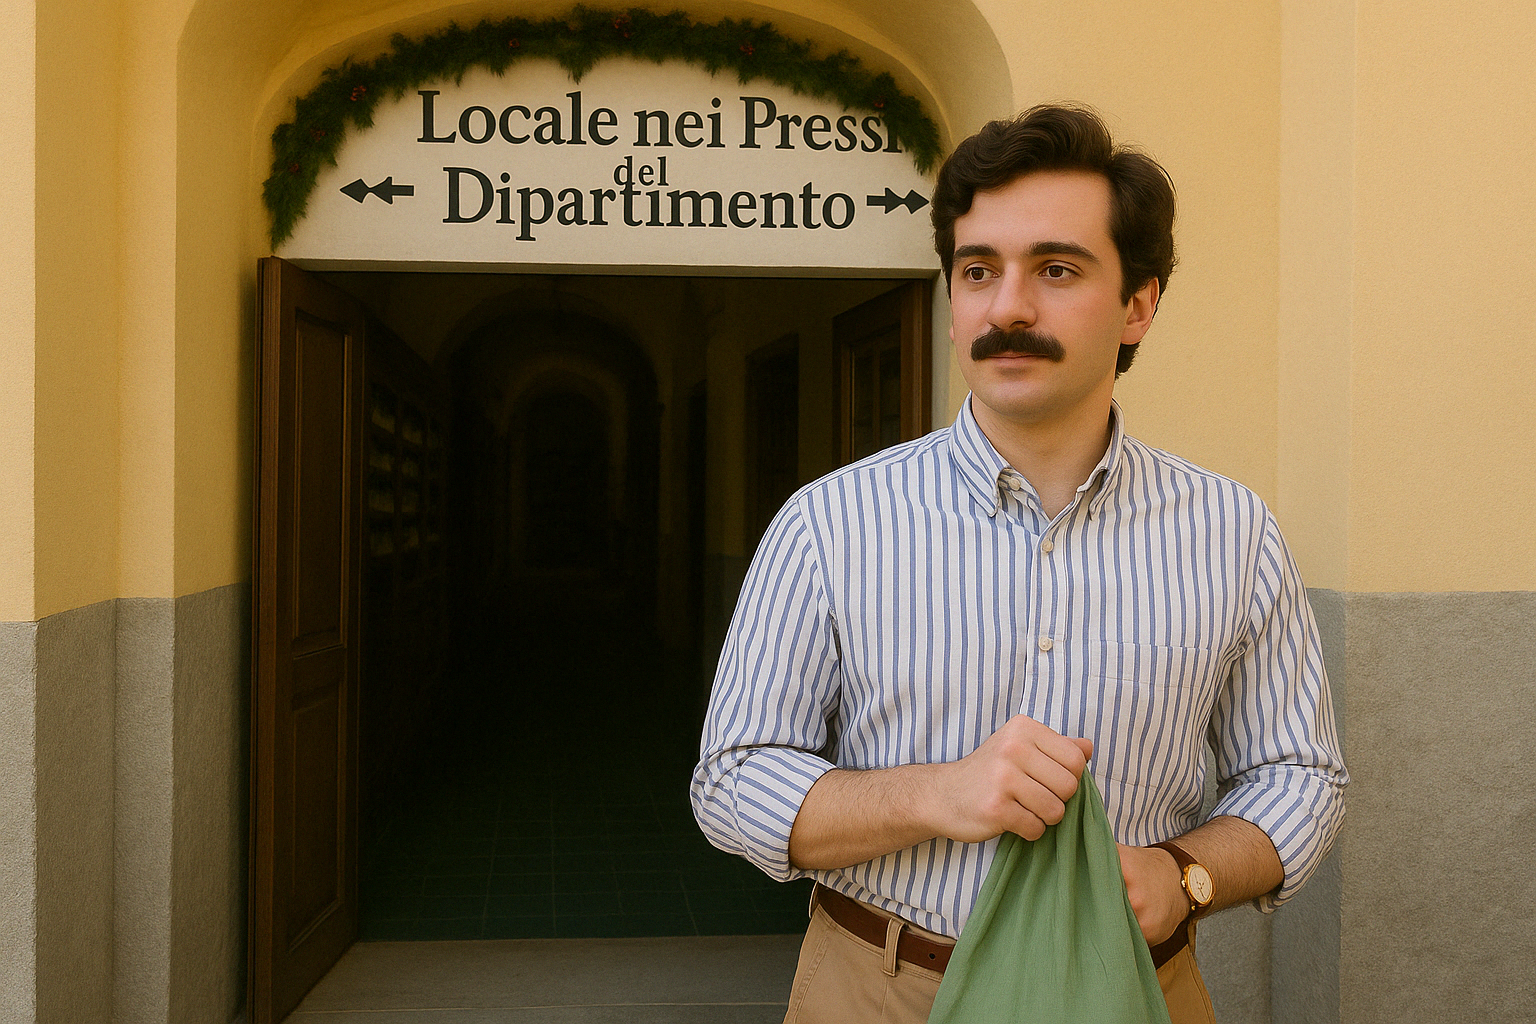
\includegraphics[width=\linewidth]{mirko.png}
\end{figure}
\end{frame}

\begin{frame}{Perché la psicometria? Il caso del dott. Mirko Marmellata}
\begin{block}{Il dott. Marmellata}
ogni giorno sceglie di comprare il pranzo al \textit{Locale nei Pressi del Dipartimento}, nonostante spenda molto di più rispetto al portarsi il pranzo da casa, e non sia mai del tutto soddisfatto della qualità e della quantità offerta.
\end{block}
\vspace{1em}
\begin{block}{Per gli standard dell'homo oeconomicus}
la sua scelta sarebbe \textbf{irrazionale}. Volendo essere gentili, la scelta ci appare comunque \textbf{non ottimale}.
\end{block}
\end{frame}

\begin{frame}{Perché la psicometria? Il caso del dott. Mirko Marmellata}
\begin{block}{Random Utility Model (RUM)}
\[
U_{ia} = V_{ia} + \varepsilon_{ia}
\]
\begin{itemize}
  \item \(U_{ia}\): utilità totale che l’individuo \(i\) associa all’alternativa \(a\);
  \item \(V_{ia}\): componente osservabile (prezzo, quantità...);
  \item \(\varepsilon_{ia}\): componente non osservata (abitudini, emozioni...).
\end{itemize}
\end{block}
\vspace{1em}
\begin{block}{Per Mirko Marmellata:}
\[
U_{\text{MM}, \text{Locale}} > U_{\text{MM}, \text{Casa}}
\]
Ciò che guida la sua preferenza è probabilmente nascosto in \(\varepsilon\).
\end{block}
\end{frame}

\begin{frame}{Perché la psicometria? Il caso del dott. Mirko Marmellata}
\begin{block}{Il ruolo della psicometria}
Permette di ``aprire'' la \(\varepsilon\) e di modellare i costrutti latenti che influenzano le decisioni.
\end{block}
\vspace{1em}
\begin{block}{Obiettivo}
Portare i fattori psicologici fuori da \(\varepsilon\) e dentro il modello, migliorando \textbf{predizione} e \textbf{comprensione}.
\end{block}
\end{frame}

\section{Breve introduzione alla teoria della misurazione}
\begin{frame}{Vietnam flashback...}
\begin{center}
   {\huge \alert{DATA GENERATING PROCESS}} 
\end{center}
\vspace{0.5cm}
\begin{itemize}
    \item Come misurare qualcosa che non possiamo osservare?
\end{itemize}
\pause
\vspace{0.5cm}
Secondo la \textbf{teoria della misurazione}, anche se non possiamo osservare direttamente un concetto teorico (come l'intelligenza), possiamo osservarne i {\it riflessi} nella realtà: comportamenti, risposte, risultati... \\
\vspace{0.5 cm}
\footnotesize
{\it Esempio:} \\
Non pesiamo l'intelligenza di una persona su una bilancia, ma possiamo inferirla da una serie di segnali: si è laureata con lode, è brava con Stata, usa parole complicate, ha letto tutti i romanzi russi dell'Ottocento... {\it Nota che molto dipende dalla nostra definizione di intelligenza!}
\end{frame}

\begin{frame}{Cosa intendiamo per misurazione}
\begin{block}{Definizione proposta:}
    Assegnazione \textit{sitematica} di un punteggio a delle entità (individui, oggetti, eventi...), in modo tale che il punteggio rappresenti una caratteristica di quelle entità.
\end{block}
\pause
\begin{itemize}
    \item Quando la caratteristica investigata è di natura psicologica, la scienza della misurazione è chiamata \textbf{psicometria}.
\end{itemize}
\end{frame}

\section{I costrutti: definizioni concettuali e operazionali}
\begin{frame}{I costrutti}
Alcune caratteristiche di interesse sono semplici da misurare: età del consumatore, altezza, peso. \\ Altre, come l’intelligenza, l’autostima o gli atteggiamenti, non possono essere osservate direttamente.
\begin{itemize}
    \item Queste variabili si chiamano \textbf{costrutti}.
\end{itemize}
\end{frame}

\begin{frame}{I costrutti}
I costrutti includono (ma non si limitano a):
    \begin{itemize}
      \item Tratti di personalità (es. estroversione)
      \item Stati emotivi (es. paura)
      \item Atteggiamenti (es. verso le certificazioni)
      \item Abilità (es. nelle materie scientifiche)
    \end{itemize}
\end{frame}

\begin{frame}{I costrutti}
  \begin{itemize}
    \item Il costrutto descrive una \textit{tendenza generale} ad agire in un certo modo, non un comportamento specifico nel momento.
    \item I costrutti sono \textbf{sintesi astratte} di processi complessi.
    \item Nessun comportamento o processo singolo può “definire” completamente il costrutto.
  \end{itemize}
\end{frame}

\begin{frame}{Definizione concettuale di un costrutto}
  \begin{block}{Cos'è una definizione concettuale?}
    Descrive i comportamenti e i processi interni che costituiscono un costrutto psicologico, e spiega come esso si relaziona ad altre variabili.
  \end{block}
  \pause
  \begin{itemize}
    \item Esempio: il \textbf{neuroticismo} può essere definito come la tendenza stabile a provare emozioni negative (ansia, rabbia, tristezza) in molteplici situazioni.
    \item Può includere anche: origine genetica, stabilità nel tempo, correlazioni con dolore fisico e sintomi somatici.
    \pause
    \item Le definizioni scientifiche differiscono da quelle del dizionario (più precise, empiricamente testabili, e aperte alla revisione).
    \item Spesso esistono più definizioni concettuali dello stesso costrutto in letteratura.
  \end{itemize}
\end{frame}

\begin{frame}{Definizione operazionale di un costrutto}
  \begin{block}{Cos'è una definizione operazionale?}
    È una definizione di un costrutto in termini di come viene misurato concretamente.
  \end{block}
  \pause
\vspace{0.8cm}
  \begin{center}
      \textbf{Definizione concettuale} \\
      \bigskip
      $\Downarrow$ \quad \textit{\small Operazionalizzazione} \quad $\Downarrow$ \\
      \bigskip
      \textbf{Definizione operazionale} \\
  \end{center}
\end{frame}

  
\begin{frame}{Definizione operazionale di un costrutto}
  Le misure operazionali si dividono in tre grandi categorie:
  \begin{enumerate}
      \item \textbf{Self-report}: l'individuo riporta i propri pensieri, emozioni o comportamenti.
      \item \textbf{Comportamentale}: si osserva e registra un comportamento.
      \item \textbf{Fisiologica}: si registrano processi biologici.
    \end{enumerate}
\end{frame}

\begin{frame}{Esempio: Risposta di disgusto verso uno yogurt “scaduto"}
\small
  Supponiamo di voler misurare la reazione di \textbf{disgusto} di un consumatore verso uno yogurt che ha superato il termine minimo di conservazione.
  \pause
      \begin{block}{Definizione concettuale}
    Il disgusto è un'emozione di base che si manifesta come risposta di evitamento verso stimoli percepiti come contaminanti, infetti o degradati. Ha una funzione evolutiva di protezione dall'ingestione di sostanze potenzialmente pericolose.
  \end{block}
  \pause
    \begin{block}{Definizioni operazionali}
  \begin{itemize}
    \item \textbf{Self-report}: il partecipante valuta quanto trova disgustosa l'idea di assaggiare il prodotto su una scala da 1 a 7.
    \item \textbf{Comportamentale}: si osserva se il partecipante rifiuta di assaggiare il prodotto.
    \item \textbf{Fisiologica}: si misura la risposta galvanica della pelle (GSR) o l'attività muscolare facciale (EMG) legata al disgusto quando chiediamo al partecipante di assaggiare il prodotto.
  \end{itemize}
\end{block}
\end{frame}

\section{I livelli di misurazione}
\begin{frame}{Livelli di misurazione}
  \begin{block}{Il livello della misurazione può essere:}
    \begin{enumerate}
      \item Nominale
      \item Ordinale
      \item A intervalli
      \item A rapporti
    \end{enumerate}
 \end{block}
Ogni livello comunica un diverso grado di informazione quantitativa, e ne determina le analisi statistiche appropriate.
\end{frame}

\begin{frame}{Nominale e Ordinale}
\begin{block}{Nominale}
    Etichette di categoria: es. genere, stato civile, etnia, colore preferito. \textbf{Non c'è nessun ordine tra le categorie.}
\end{block}
\pause
\begin{block}{Ordinale}
    Le categorie hanno un ordine (es. “molto soddisfatto", “soddisfatto", “insoddisfatto") \textbf{ma non è possibile assumere che le distanze tra le categorie siano uguali.} \\
    \pause
    \centering
    \vspace{0.5em}
    \begin{tikzpicture}[x=2cm,y=1cm]
  \fill[blue!30] (-1,-0.1) rectangle (0,2.2);     
  \fill[blue!70] ( 0,-0.1) rectangle (1,3.0);     
  \fill[blue!10] ( 1,-0.1) rectangle (2,1.5);     
  \node[font=\large\bfseries] at (-0.5,1.1) {2};
  \node[font=\large\bfseries] at ( 0.5,1.8) {1};
  \node[font=\large\bfseries] at ( 1.5,0.75) {3};
\draw[thick] (-1,-0.1) -- (2,-0.1);
    \pause
  \node at (-0.5,2.6) {01:00:26};
  \node at ( 0.5,3.4) {00:59:42};
  \node at ( 1.5,1.9) {01:00:37};
\end{tikzpicture}
\end{block}
\end{frame}

\begin{frame}{A Intervalli e a Rapporti}
  \begin{block}{A Intervalli}
  Differenze numeriche con significato coerente: es. gradi Celsius. \\
  La distanza tra 12°C e 22°C è la stessa che separa 22°C da 32°C. Però...
    \begin{itemize}
      \item \textbf{Nessun vero zero:} 0°C non significa “assenza di temperatura".
      \item Quindi \textbf{non ha senso parlare di “doppio” o “metà”:} a 30°C non fa il doppio del caldo di 15°C.
    \end{itemize}
  \end{block}
  \pause
  \begin{block}{A Rapporti}
  Come gli intervalli, ma con lo zero che indica l'\textbf{origine assoluta}. \\
    \begin{itemize}
      \item Permette confronti di proporzione: 100 kg è il doppio di 50 kg.
      \item Es.: altezza, peso, reddito, temperatura in Kelvin.
    \end{itemize}
  \end{block}
\end{frame}

\begin{frame}{Ricapitolando}
    \centering
    Operazioni possibili con le diverse scale di misura: \\
    \vspace{1em}
    \begin{tabular}{lcccc}
    \toprule
      \textbf{Livello} & \textbf{$=$ $\neq$} & \textbf{$>$ $<$} & \textbf{$+$ $-$} & \textbf{$\times$ $\div$} \\
      \midrule
      Nominale & \checkmark & & & \\
      Ordinale & \checkmark & \checkmark & & \\
      A Intervalli & \checkmark & \checkmark & \checkmark & \\
      A Rapporti & \checkmark & \checkmark & \checkmark & \checkmark \\
      \bottomrule
    \end{tabular}
\end{frame}

\section{Il questionario}
\begin{frame}{La seconda rivoluzione copernicana?}
\huge
    \[
      \Delta x \cdot \Delta p_x \;\ge\; \frac{\hbar}{2}
    \]
\end{frame}

\begin{frame}{La seconda rivoluzione copernicana?}
    \[
      \Delta x \cdot \Delta p_x \;\ge\; \frac{\hbar}{2}
    \]
\begin{block}{Principio di indeterminazione}
\small
    Enunciato da \textbf{Werner Heisenberg} nel 1927, rappresenta un concetto cardine della meccanica quantistica e ha sancito una radicale rottura rispetto alle leggi della meccanica classica. \\
    \smallskip
    Non possiamo conoscere con precisione assoluta, simultaneamente, la posizione e la velocità di una particella: \textbf{l’atto stesso di misurare qualcosa lo cambia}. Non è un problema di strumenti imperfetti, ma una caratteristica fondamentale della natura quantistica.
\end{block}
\end{frame}

\begin{frame}{Il questionario}
    Il questionario è uno strumento \textbf{self-report} utilizzato per raccogliere informazioni di natura quantitativa e/o qualitativa. Poiché viene generalmente compilato in autonomia dal partecipante, può generare l'impressione che il ricercatore sia estraneo al processo; in realtà, quest'ultimo è il solo responsabile del \\
    \vspace{1em}
    \pause
    \huge\centering
    \alert{DATA GENERATING PROCESS}
\end{frame}

\begin{frame}{Il questionario}
\begin{block}{Il partecipante}
    non è un database da cui estrarre dati, ma un \textbf{soggetto attivo} che utilizza diversi \textbf{fattori contestuali}, diversi dal contenuto delle domande, per dare significato al questionario che sta compilando. Alcuni effetti contestuali: \\
    \begin{itemize}
        \item Il modo in cui viene presentato il questionario.
        \item L’identità del ricercatore e dell’ente di ricerca.
        \item Le alternative di risposta.
        \item L'ordine delle domande.
    \end{itemize}
\end{block}
\end{frame}

\begin{frame}{Esempio: Effetto dell'ordine}
\textit{Strack et al. (1988)  hanno chiesto ad alcuni studenti universitari sia quanto fossero soddisfatti della loro vita in generale sia con quale frequenza uscissero con qualcuno.} \\
\vspace{1em}
\centering
\begin{tabular}{l|lclc}
    \toprule
   Ordine 1 & Soddisfazione & $\rightarrow$ & Appuntamenti & $r$ = -.12 \\
   \midrule
   \pause
   Ordine 2 & Appuntamenti & $\rightarrow$ & Soddisfazione & $r$ = +.66 \\
   \bottomrule
\end{tabular}
\vspace{0.3cm}
\begin{block}{Possibili soluzioni?}
\pause
\begin{itemize}
    \item \textbf{Distanziare} le domande nel questionario.
    \pause
    \item \textbf{Randomizzare} la presentazione delle domande.
    \pause
    \item \textbf{Fare entrambe le cose}.
\end{itemize}
\end{block}
\end{frame}

\begin{frame}{Processi cognitivi nella risposta a un item}
Quanti drink alcolici consumi in una giornata tipo? \\
\vspace{0.2cm}
\begin{tabular}{ll}
    $\bigcirc$ & Molto più della media \\
    $\bigcirc$ & Un po' più della media \\
    $\bigcirc$ & Nella media \\
    $\bigcirc$ & Un po' meno della media \\
    $\bigcirc$ & Molto meno della media \\
\end{tabular}
\vspace{1em}
\\ \textit{Anche quando poniamo una domanda all'apparenza banale, il processo di risposta può essere complesso, aperto a intepretazioni e manipolazioni.}
\end{frame}

\begin{frame}{Processi cognitivi nella risposta a un item}
  \resizebox{\textwidth}{!}{%
    \begin{tikzpicture}[
      process/.style={
        rectangle, 
        draw=blue, very thick, 
        rounded corners, 
        minimum width=3cm, 
        minimum height=2cm, 
        align=center
      },
      arrow/.style={
        -{Stealth[length=3mm,width=2mm]}, 
        thick
      }
    ]
      \node[process] (comprehension) {Comprensione \\ della domanda};
      \node[process, right=of comprehension] (retrieval) {Recupero \\ delle informazioni};
      \node[process, right=of retrieval] (judgment) {Formazione \\ del giudizio};
      \node[process, right=of judgment] (response) {Formattazione \\ della risposta};
      \draw[arrow] (comprehension) -- (retrieval);
      \draw[arrow] (retrieval) -- (judgment);
      \draw[arrow] (judgment) -- (response);
    \end{tikzpicture}%
  }
\end{frame}

\begin{frame}{Modello BORIS}
    Il modello BORIS\footnote{\scriptsize{Denominato BRUSO in \cite{jhangiani2019research}}} offre cinque principi utili per la stesura di domande efficaci nei questionari.\\
    \vspace{1em}
    \begin{table}[]
        \centering
    \begin{tabular}{cc}
    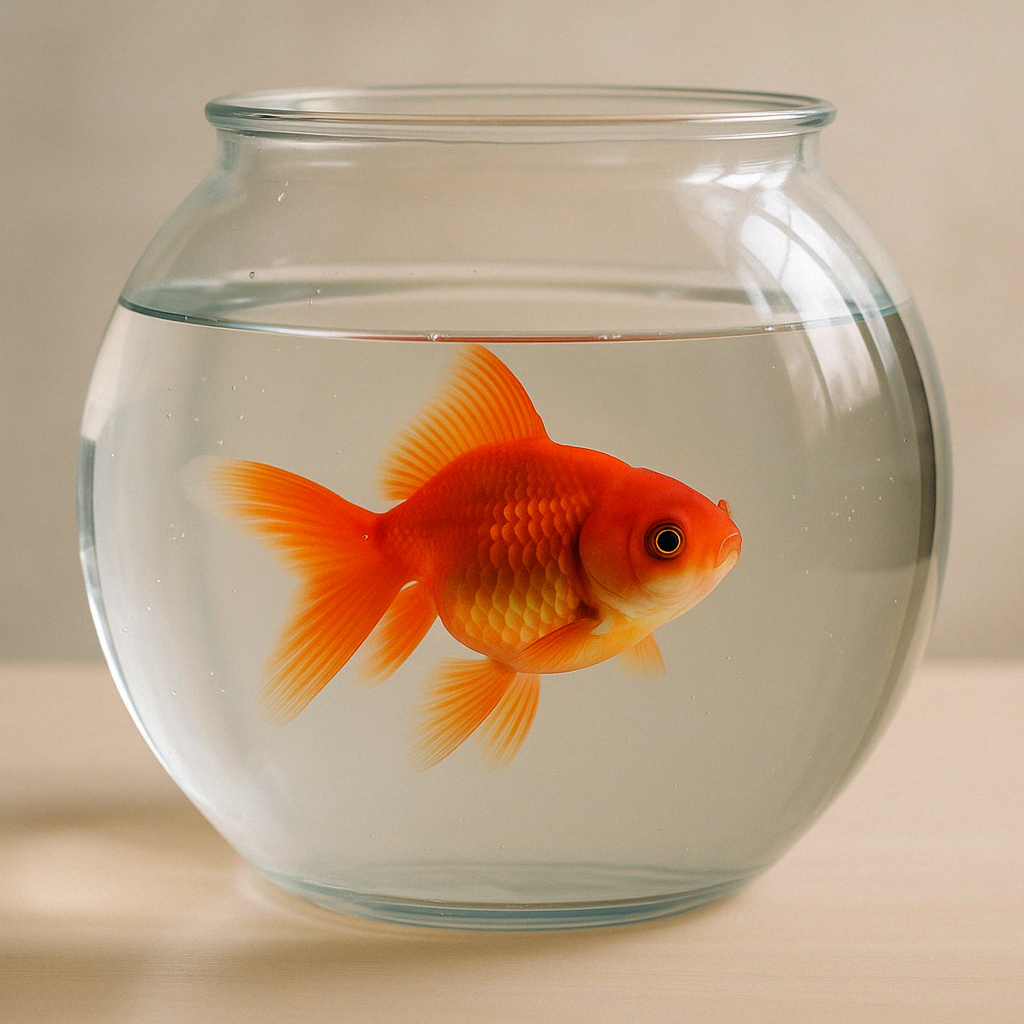
\includegraphics[width=0.45\linewidth]{boris.png} & 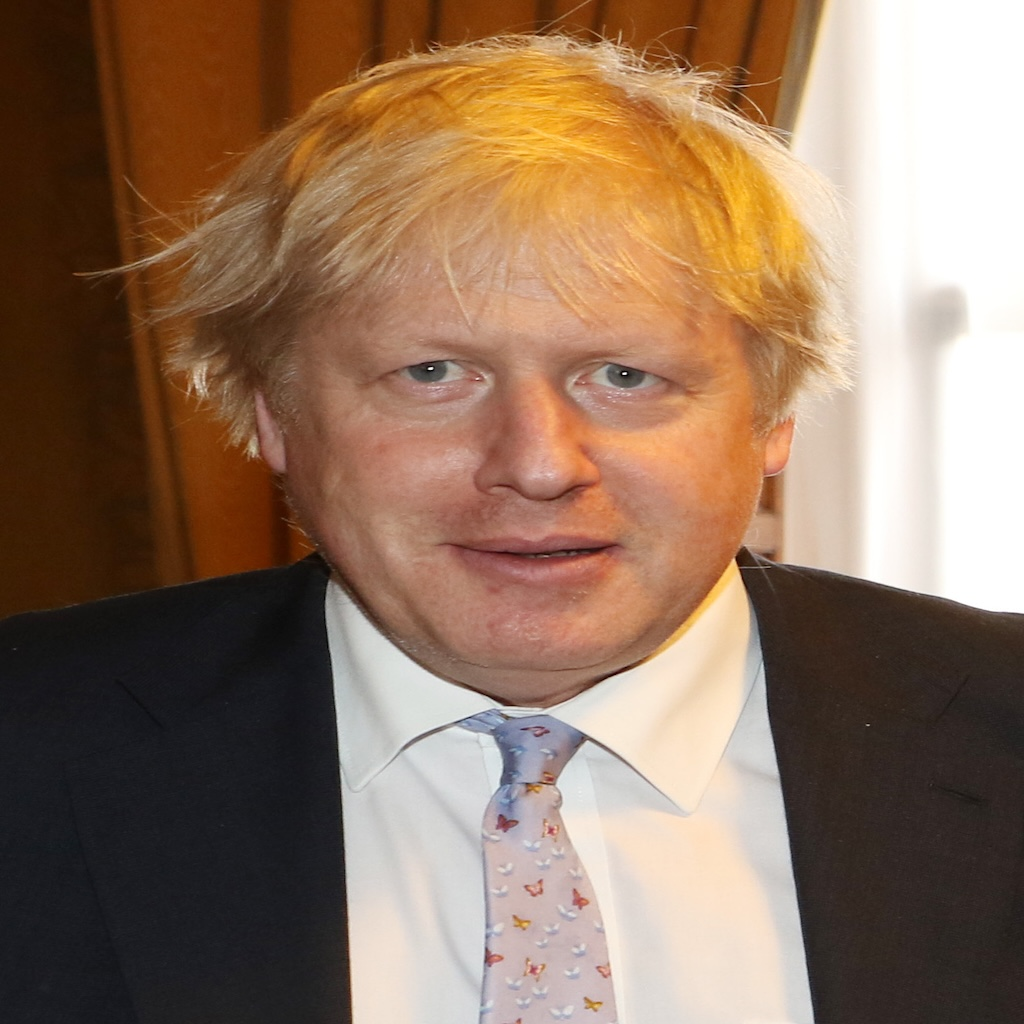
\includegraphics[width=0.45\linewidth]{boris2.jpg} \\
    \footnotesize{Pesce rosso} & \footnotesize{Ex primo ministro del Regno Unito}
    \end{tabular}
    \end{table}
\end{frame}

\begin{frame}{Modello BORIS}
  \scriptsize
  \centering
  \begin{tabular}{lp{4cm}p{3.5cm}}
    \toprule
    \textbf{Criterio} & \textbf{Poco efficace} & \textbf{OK} \\
    \midrule
    \textbf{B}revità & “Ti è mai capitato, nel corso della tua vita, di imbatterti nel concetto di agricoltura sociale?” & “Hai mai sentito parlare di agricoltura sociale?” \\
    \\
    \textbf{O}ggettività & “Quanto sostieni la certificazione etica NoCap?” & “Qual è la tua opinione sulla certificazione NoCap?” \\
    \\
    \textbf{R}ilevanza & “Per quale partito hai votato alle scorse elezioni politiche?” & Non includere la domanda se non è chiaramente rilevante. \\
    \\
    \textbf{I}nequivocabilità & “Sei una persona salutista?” & “Controlli abitualmente le etichette nutrizionali quando fai la spesa?” \\
    \\
    \textbf{S}pecificità & “Hai mai sentito parlare di produzione integrata e di SQNPI?” & “Hai mai sentito parlare di produzione integrata?” \\
    \bottomrule
  \end{tabular}
\end{frame}

\section{Cosa sono gli atteggiamenti e come misurarli}
\begin{frame}{Atteggiamenti $\neq$ Attitudini}
    \begin{block}{Cosa sono gli atteggiamenti?}
        Dal 1918 sono state coniate oltre 500 definizioni di atteggiamenti! \\
        Dalle diverse definizioni emerge una componente di \textbf{valutazione} (positiva-negativa) del soggetto rispetto a un oggetto: \\
        \pause
        \small
    \begin{itemize}
        \item Allport (1954) definisce l’atteggiamento come uno stato mentale, organizzato grazie all’esperienza, che esercita un’influenza sulle risposte dell’individuo nei confronti di tutti gli oggetti e le situazioni con cui è in relazione.
        \item Per la Social Cognition (Fazio, 1986) l’atteggiamento è una struttura cognitiva costituita dall’associazione in memoria tra la rappresentazione dell’oggetto e la sua valutazione.
        \item Mayers (2021) definisce l’atteggiamento come una valutazione favorevole o sfavorevole verso qualcosa o qualcuno, spesso radicata nelle proprie credenze ed esibita nei sentimenti e nel comportamento intenzionale.
    \end{itemize}
    \end{block}
\end{frame}

\begin{frame}{Atteggiamenti $\neq$ Attitudini}
    \begin{block}{A cosa servono gli atteggiamenti?}
        Katz (1960) suggerisce che gli atteggiamenti possono servire quattro funzioni principali: \\
        \small
    \begin{enumerate}
        \item \textbf{Utilitaristica}: l'atteggiamento verso un certo oggetto si sviluppa per raggiungere un beneficio o evitare un effetto negativo (es. Atteggiamento positivo verso la dieta vegana perché percepita come più salutare);
        \item \textbf{Espressione del valore}: per esprimere valori e \textit{self-concept} individuali (es. Atteggiamento positivo verso la dieta vegana per esprimere i propri \textit{valori etici});
        \item \textbf{Difesa del Sé}: per difendere una mancanza percepita a livello identitario (es. Atteggiamento negativo verso la dieta vegana, da parte di un uomo, perché mangiare l'insalata è poco virile); 
        \item \textbf{Cognitiva}: per rispondere al bisogno di ordine, equilibrio e coerenza...
    \end{enumerate}
    \end{block}
\end{frame}

\begin{frame}{Atteggiamenti $\neq$ Attitudini}
    \footnotesize
    \begin{block}{La Balance Theory (Heider, 1946)}
        si fonda proprio sul principio di coerenza cognitiva, e formula l'esistenza di strutture attitudinali triadiche che tendono alla ristrutturazione cognitiva in caso di disequilibrio. \\
        La struttura triadica è data da almeno due persone e al massimo un oggetto. A seconda degli atteggiamenti con cui si associano gli uni agli altri possono rappresentare strutture equilibrate o disequilibrate che tenderanno, perciò, a un cambiamento. \\
        \vspace{0.5em}
        \centering
        \begin{tikzpicture}
            \draw[blue, ultra thick] (4,0) -- (8,0) -- (6,2) -- cycle;
            \node at (4.7,1.3) {\textbf{\scriptsize+}};
            \node at (7.3,1.3) {\textbf{\scriptsize+}};
            \node at (6,-0.4) {\textbf{\scriptsize –}};
            \node at (4,-0.4) {\textbf{\scriptsize Mirko}};
            \node at (8,-0.4) {\textbf{\scriptsize Montagna}};
            \node at (6,2.4) {\textbf{\scriptsize Francesca}};
        \end{tikzpicture}
        \\
        \vspace{0.5em}
        \textit{\scriptsize Una triade è considerata in equilibrio quando il prodotto dei segni è positivo.} \\
    \end{block}
\end{frame}

\begin{frame}{Atteggiamenti $\neq$ Attitudini}
    \begin{block}{La Balance Theory nel marketing}
        Molte aziende ricorrono a testimonial amati dal pubblico per promuovere la formazione di un atteggiamento positivo verso il proprio prodotto o servizio.  \\
        \vspace{0.5em}
        \centering
        \pause
        \begin{tikzpicture}
            \draw[blue, ultra thick] (4,0) -- (8,0) -- (6,2) -- cycle;
            \node at (4.7,1.3) {\textbf{\scriptsize +}};
            \node at (7.3,1.3) {\textbf{\scriptsize ?}};
            \node at (6,-0.4) {\textbf{\scriptsize +}};
            \node at (4,-0.4) {\textbf{\scriptsize Chiara Ferragni}};
            \node at (8,-0.4) {\textbf{\scriptsize Pandoro Balocco}};
            \node at (6,2.4) {\textbf{\scriptsize Mirko Marmellata}};
        \end{tikzpicture}
    \end{block}
\end{frame}

\begin{frame}{Atteggiamenti $\neq$ Attitudini}
    \begin{block}{Alcune caratteristiche di base:}
        \small
        \begin{itemize}
            \item Gli atteggiamenti sono relativamente permanenti nel tempo e trasversali alle situazioni.
            \item Gli atteggiamenti implicano sempre un certo grado di astrazione e risultano essere generalizzabili a più situazioni, oggetti o condizioni.
            \item Gli atteggiamenti hanno sempre una rilevanza sociale poiché influiscono sulla percezione della persona in relazione agli altri, sulle preferenze e sui comportamenti.
        \end{itemize}
        \textbf{L’atteggiamento è quindi un mezzo utile per prevedere i comportamenti di consumo.}
    \end{block}
\end{frame}

\tikzset{
  block/.style = {draw=blue!80, fill=blue!10, very thick, ellipse, minimum height=2cm, minimum width=3cm, align=center}, arrow/.style = {thick, ->, >=Stealth}
}

\begin{frame}{Teoria dell'Azione Ragionata (Fishbein \& Ajzen, 1975)}
\resizebox{\textwidth}{!}{%
\centering
\begin{tikzpicture}[node distance=1.5cm, auto]
  \node[] (pbc) {};
  \node[block, above=of pbc] (att) {Atteggiamento \\ verso il \\ comportamento};
  \node[block, below=of pbc] (ns) {Norme soggettive};
  \node[block, right=of pbc] (int) {Intenzione \\ comportamentale};
  \node[block, right=of int] (beh) {Comportamento};
  \draw[arrow] (att) -- (int);
  \draw[arrow] (ns)  -- (int);
  \draw[arrow] (int) -- (beh);
\end{tikzpicture}
}
\end{frame}

\begin{frame}{Teoria del Comportamento Pianificato (Ajzen, 1991)}
\resizebox{\textwidth}{!}{%
\centering
\begin{tikzpicture}[node distance=1.5cm, auto]
  \node[block] (pbc) {Controllo \\ comportamentale \\ percepito};
  \node[block, above=of pbc] (att) {Atteggiamento \\ verso il \\ comportamento};
  \node[block, below=of pbc] (ns) {Norme soggettive};
  \node[block, right=of pbc] (int) {Intenzione \\ comportamentale};
  \node[block, right=of int] (beh) {Comportamento};
  \draw[arrow] (att) -- (int);
  \draw[arrow] (pbc) -- (int);
  \draw[arrow] (ns)  -- (int);
  \draw[arrow] (int) -- (beh);
\end{tikzpicture}
} \\
\vspace{1em}
\footnotesize\centering\it Il 63\% dei professori qui ha almeno una pubblicazione basata sulla TPB!
\end{frame}

\begin{frame}{Misurare gli atteggiamenti: Scala di Likert}
\begin{columns}[c]
  \column{0.55\textwidth}
  \begin{figure}
    \centering
    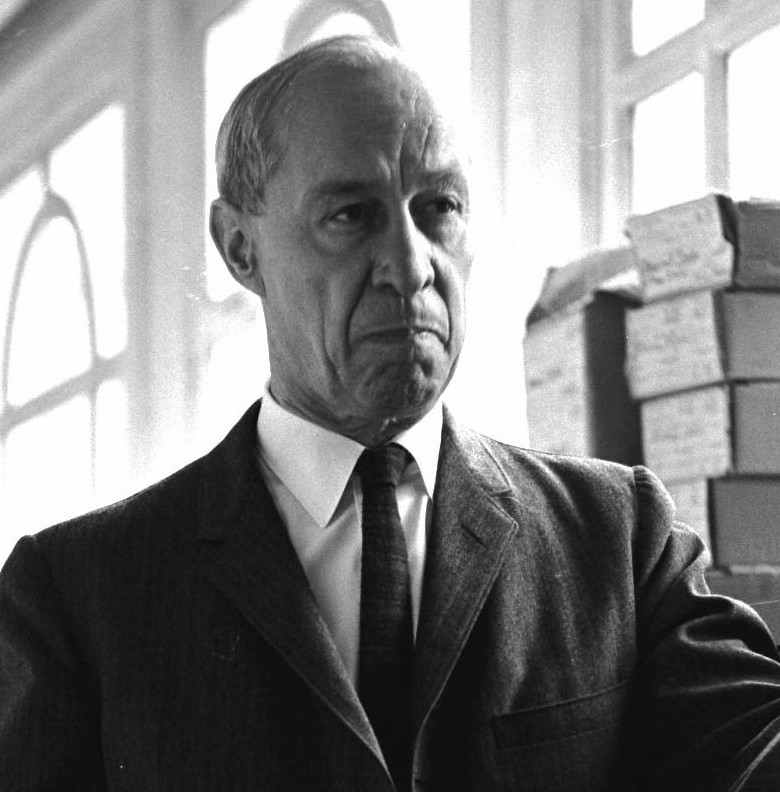
\includegraphics[width=\linewidth]{likert.jpg}
    \caption{Rensis Likert (1903–1981)}
  \end{figure}
  \column{0.45\textwidth}
  \begin{block}{Scala di Likert}
    \small
    La scala di Likert, o \textit{scala a somma di punteggi}, è molto utilizzata perché di facile costruzione: vengono considerate una serie di affermazioni (\textit{item}) semanticamente collegate agli atteggiamenti da studiare, e si costruiscono delle batterie di domande sulle quali l’intervistato è chiamato ad esprimere il proprio grado di accordo o disaccordo.
  \end{block}
\end{columns}
\end{frame}

\begin{frame}{Esempio: Neofobia verso le tecnologie alimentari}
  \begin{block}{Food Technology Neophobia Scale (Cox \& Evans, 2008)}
    La FTNS è uno strumento popolare per misurare la neofobia verso le tecnologie alimentari e si basa sulla scala di Likert.
  \end{block}
  \vspace{0.3cm}
  \small
  \begin{tabular}{l l}
    \textbf{FTNS 1:} & Non ho ragione di provare cibi altamente tecnologici \\
    & perché quelli che mangio sono già abbastanza buoni \\
    \textbf{FTNS 2:} & Le nuove tecnologie alimentari sono qualcosa di cui \\
    & sono incerto \\
    \textbf{FTNS 3:} & I nuovi prodotti alimentari non sono più salutari dei \\ 
    & cibi tradizionali \\
    \textbf{(...)}
  \end{tabular}
  \vspace{0.2cm}
  \begin{center}
    \footnotesize
    \begin{tabular}{ccccc}
      \toprule
      \textit{Fortemente} & \textit{In disaccordo} & \textit{Né d'accordo} & \textit{D'accordo} & \textit{Fortemente} \\
      \textit{in disaccordo} &  & \textit{né in disaccordo} &  & \textit{d'accordo} \\
      \midrule
      $\bigcirc$ & $\bigcirc$ & $\bigcirc$ & $\bigcirc$ & $\bigcirc$ \\
      \bottomrule
    \end{tabular}
  \end{center}
\end{frame}

\begin{frame}{Esempio: Neofobia verso le tecnologie alimentari}
  \begin{block}{Food Technology Neophobia Scale (Cox \& Evans, 2008)}
    La FTNS è uno strumento popolare per misurare l'avversione verso le nuove tecnologie alimentari e si basa sulla scala di Likert.
  \end{block}
  \vspace{0.3cm}
  \small
  \begin{tabular}{l l}
    \textbf{FTNS 1:} & Non ho ragione di provare cibi altamente tecnologici \\
    & perché quelli che mangio sono già abbastanza buoni \\
    \textbf{FTNS 2:} & Le nuove tecnologie alimentari sono qualcosa di cui \\
    & sono incerto \\
    \textbf{FTNS 3:} & I nuovi prodotti alimentari non sono più salutari dei \\ 
    & cibi tradizionali \\
    \textbf{(...)}
  \end{tabular}
  \vspace{0.2cm}
  \begin{center}
    \footnotesize
    \begin{tabular}{ccccc}
      \toprule
      \textit{Fortemente} & \textit{In disaccordo} & \textit{Né d'accordo} & \textit{D'accordo} & \textit{Fortemente} \\
      \textit{in disaccordo} &  & \textit{né in disaccordo} &  & \textit{d'accordo} \\
      \midrule
      1 & 2 & 3 & 4 & 5 \\
      \bottomrule
    \end{tabular}
  \end{center}
\end{frame}

\begin{frame}{Misurare gli atteggiamenti: Differenziale semantico}
\begin{columns}[c]
  \column{0.55\textwidth}
  \begin{figure}
    \centering
    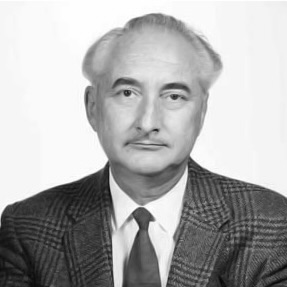
\includegraphics[width=\linewidth]{osgood.jpg}
    \caption{Charles E. Osgood (1916–1991)}
  \end{figure}
  \column{0.45\textwidth}
  \begin{block}{Scala di Osgood}
    \small
    La scala di Osgood, o \textit{differenziale semantico}, si basa su coppie di aggettivi opposti tra loro. Il rispondente indica la propria posizione lungo un continuum, rivelando così la propria rappresentazione mentale del concetto target.
  \end{block}
\end{columns}
\end{frame}

\begin{frame}{Target di esempio: “Stata”}
  \begin{center}
    \small
    \begin{tabular}{|c|c|c|c|c|c|c|c|c|}
    \hline
      & -3 & -2 & -1 & 0 & 1 & 2 & 3 & \\
      \hline
      \text{Aggressivo} & $\bigcirc$ & $\bigcirc$ & $\bigcirc$ & $\bigcirc$ & $\bigcirc$ & $\bigcirc$ & $\bigcirc$ & \text{Pacifico} \\
      \hline
      \text{Sgradevole}  & $\bigcirc$ & $\bigcirc$ & $\bigcirc$ & $\bigcirc$ & $\bigcirc$ & $\bigcirc$ & $\bigcirc$ & \text{Piacevole} \\
      \hline
      \text{...} & $\bigcirc$ & $\bigcirc$ & $\bigcirc$ & $\bigcirc$ & $\bigcirc$ & $\bigcirc$ & $\bigcirc$ & \text{...} \\
      \hline
    \end{tabular}
  \end{center}
  \pause
  \begin{figure}
    \centering
    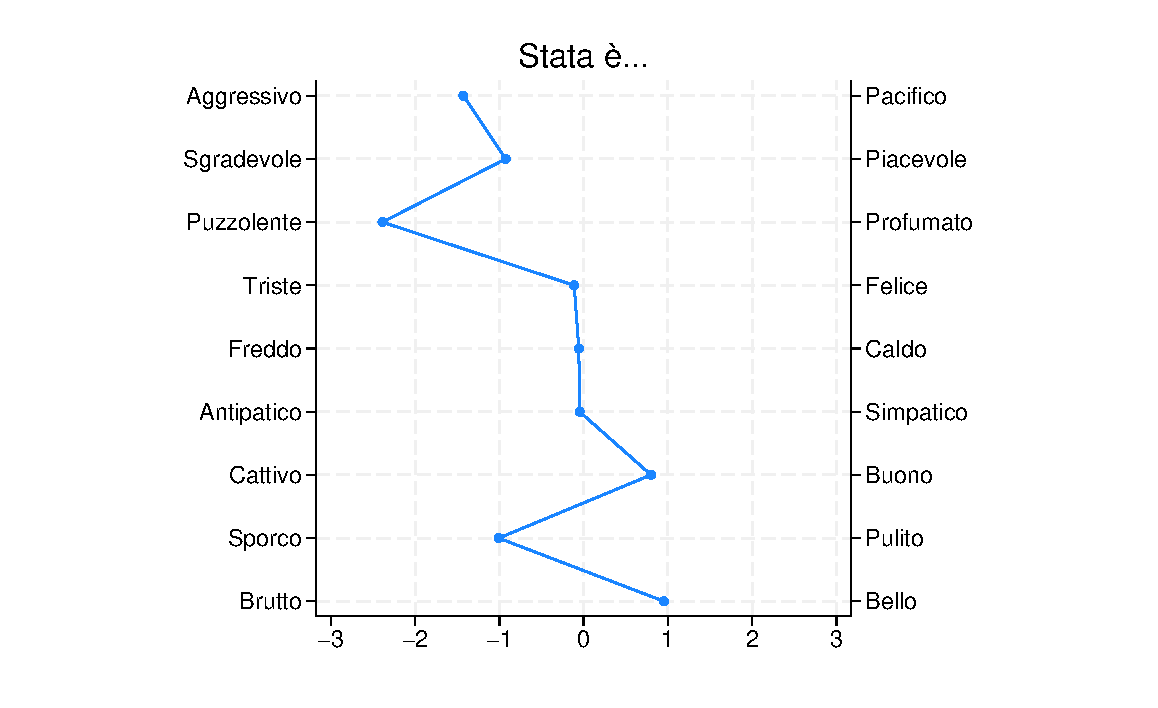
\includegraphics[width=0.9\linewidth]{osgood.eps}
  \end{figure}
\end{frame}

\end{document}